\documentclass[12pt,compress]{beamer}
\usepackage[utf8x]{inputenc}
\usepackage[ngerman]{babel}
\usepackage{color}
\usepackage{hyperref}
\usepackage{kmath,kerkis}
\usepackage{listings}

\usetheme{Boadilla}
\setbeamertemplate{footline}

\usecolortheme{lily}
\usefonttheme{serif}
\useinnertheme{circles}
\setbeamercovered{transparent}
\beamertemplatenavigationsymbolsempty

\definecolor{darkgreen}{rgb}{0,0.5,0}

\hypersetup{
    bookmarks=true,
    unicode=true,
    pdftoolbar=true,
    pdfmenubar=true,
    pdffitwindow=false,
    pdfstartview={FitH},
    pdftitle={Dark Corners of C},
    pdfauthor={Michael Hartmann},
    pdfcreator={vim},
    pdfproducer={pdflatex},
    pdfkeywords={C} {undefined behavior} {LIT} {Linux} {Infotag} {Augsburg} {LUGA},
    pdfnewwindow=true,
    colorlinks=true,
    linkcolor=black,
    citecolor=green,
    filecolor=magenta,
    urlcolor=darkgreen
}


\title{Dark Corners of C}
\institute{16. Augsburger Linux-Infotag}
\author{Michael Hartmann}
\date{22. April 2017}


\titlegraphic{
\includegraphics[scale=0.2]{images/logo.png}}

\begin{document}

\begin{frame}
    \titlepage
\end{frame}

\section{Einleitung}
\frame {
    \frametitle{Mein Weg zu C}
    
    \begin{center}
    \only<1>
    {
    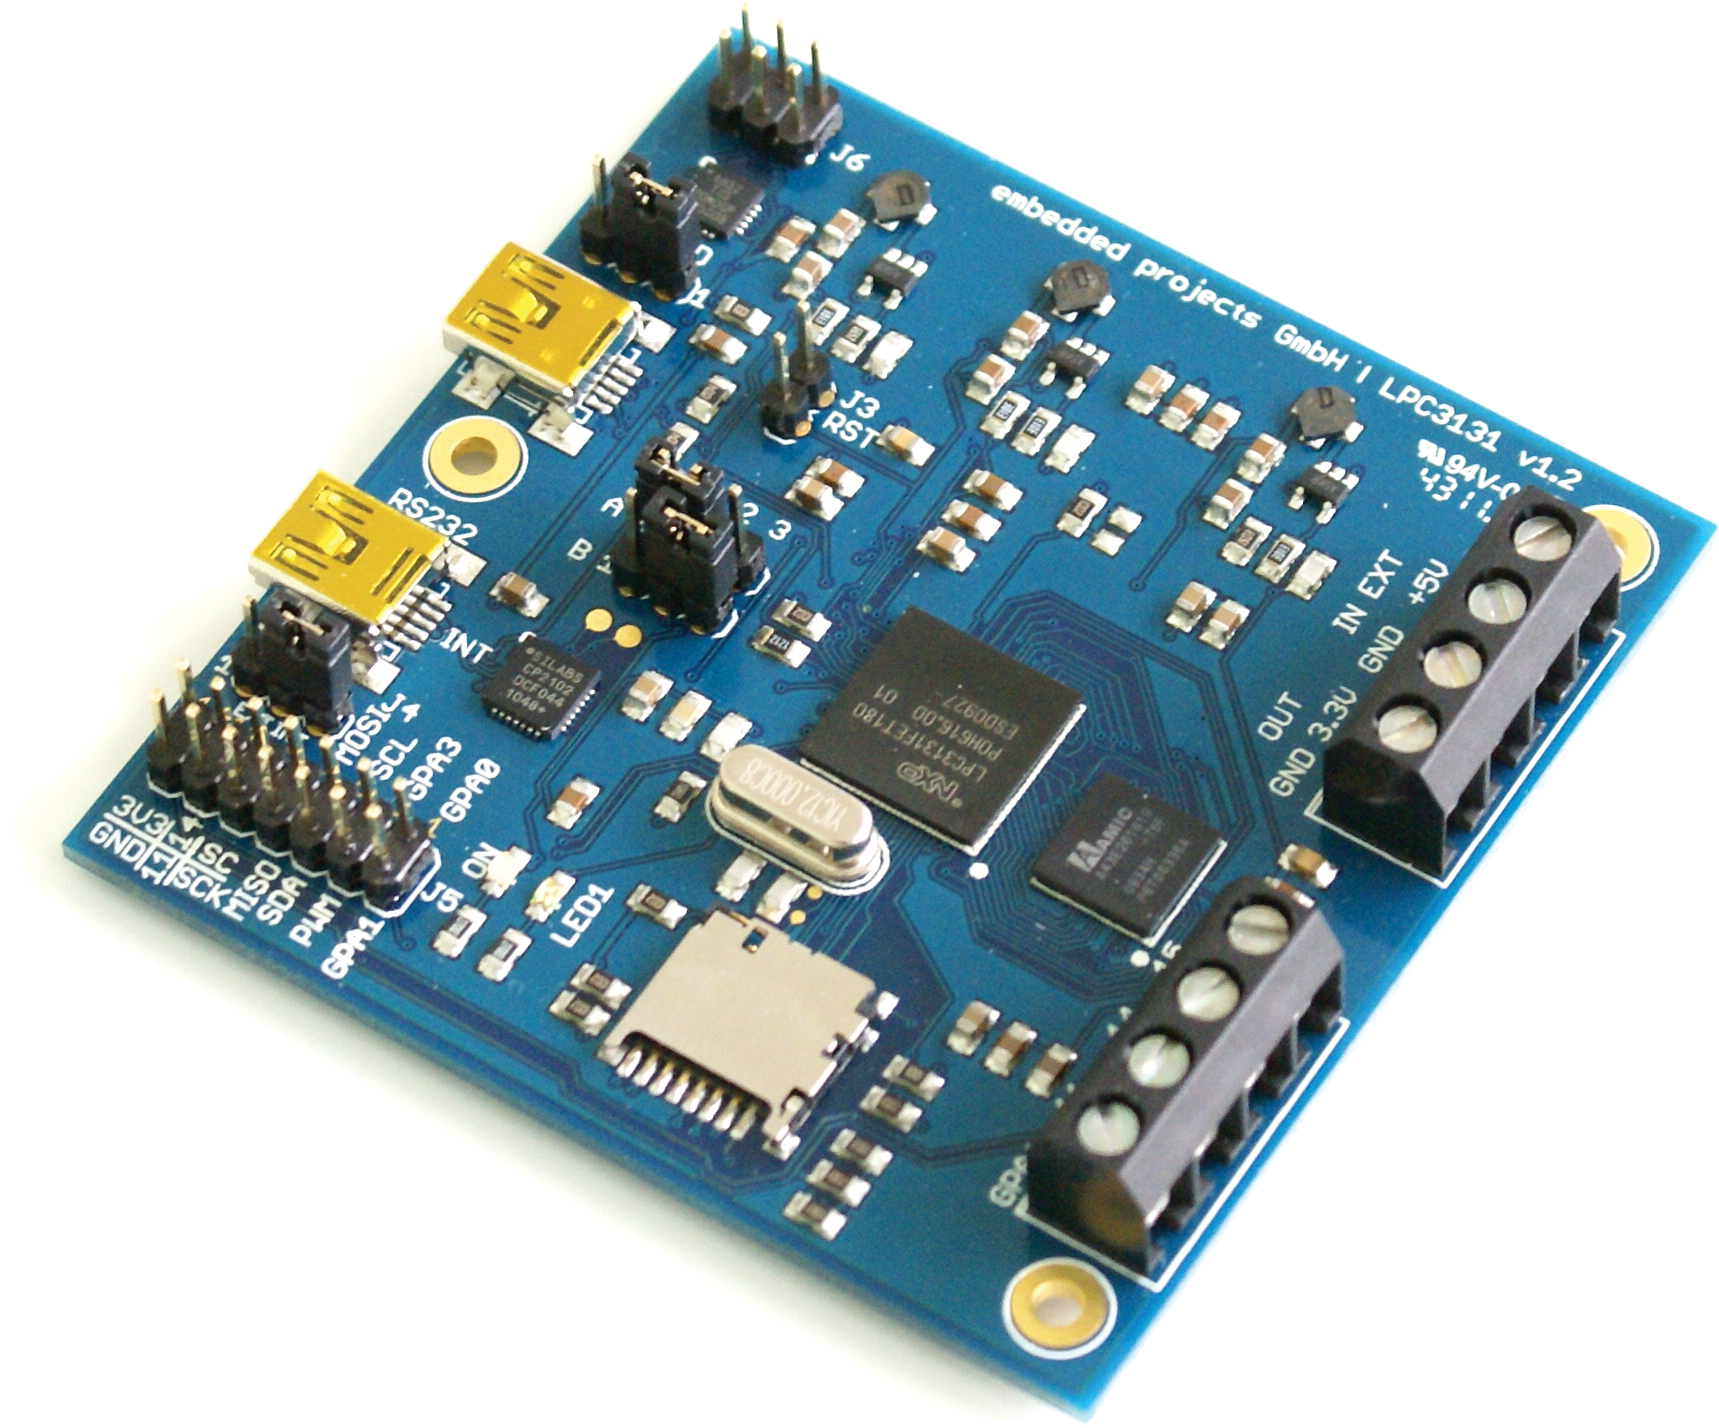
\includegraphics[scale=0.4]{images/gnublin.png}
    }

    \only<2>
    {
    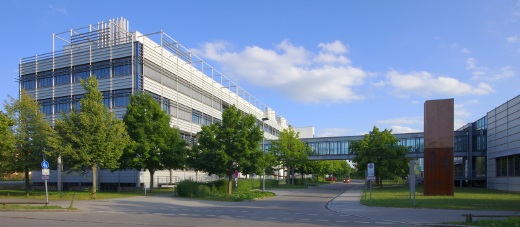
\includegraphics[scale=0.6]{images/physik.jpg}
    }
    \end{center}
}

\frame {
    \frametitle{TIOBE Programming Community Index}

    \begin{center}
    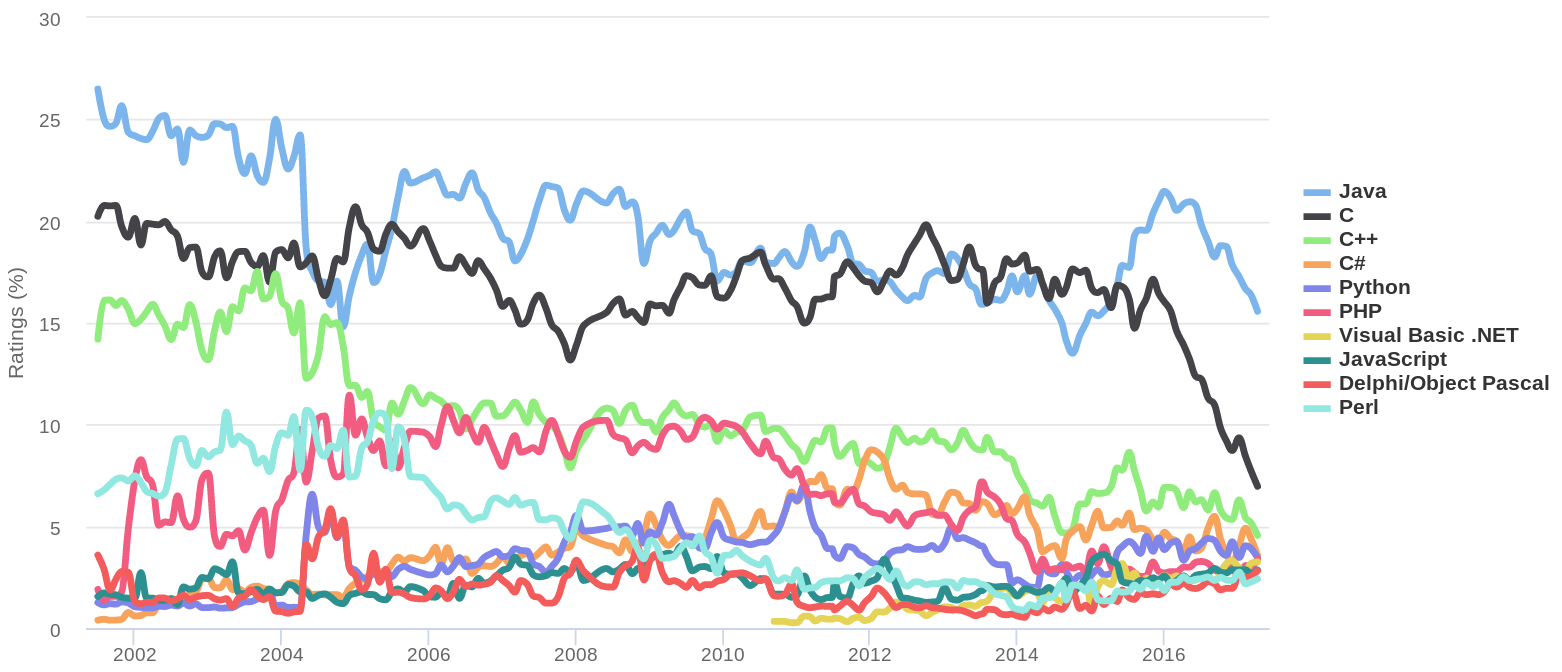
\includegraphics[scale=0.3]{images/tiobe.png}
    \end{center}
}

\frame {
    \frametitle{The \textit{spirit} of C}

    \begin{enumerate}
    \item Vertraue dem Programmierer
    \item Sprachumfang klein und einfach
    \item schnell
    \item portabel
    \end{enumerate}
}

\section{Die Sprache}

\frame {
    \frametitle{Keywords}

\texttt{{\only<2->{\color{red}}auto}
    break
    case
    char
    const
    continue
    default
    do
    double
    else
    enum
    extern
    float
    for
    goto
    if
    int
    long
    register
    return
    short
    {\only<3>{\color{red}}signed}
    sizeof
    static
    struct
    switch
    typedef
    union
    unsigned
    void
    volatile
    while 
    }
}

\begin{frame}
    \frametitle{VLA}

    Variable length arrays
    \begin{itemize}
    \item mandatory in C99
    \item optional in C11 (?!)
    \end{itemize}

    \vfill

    \only<2,3>
    {{\it For such an object that does have a variable length array type, its
    lifetime extends from the declaration of the object until execution of the
    program leaves the scope of the declaration. If the scope is entered
    recursively, a new instance of the object is created each time. The initial
    value of the object is indeterminate.}} 

    \vfill

    \only<3>
    {
    Stack?

    Heap?
    }

\end{frame}

\begin{frame}[fragile]
    \frametitle{VLA}

\begin{lstlisting}[language=C,basicstyle=\ttfamily,keywordstyle=\color{red}]
double sum(size_t nmax)
{
    double sum = 0, buf[nmax];

    for(size_t i = 0; i < nmax; i++)
        buf[i] = 1./(1+i);

    for(size_t i = 0; i < nmax; i++)
        sum += buf[i];

    return sum;
}

sum(1000);     // 5.18738...
sum(10000000); // Segmentation Fault
\end{lstlisting}
\end{frame}


\begin{frame}[fragile]
\frametitle{Macros}

\begin{lstlisting}[language=C,basicstyle=\ttfamily,keywordstyle=\color{red}]
#define SQUARE(x) x*x

SQUARE(2+1);
\end{lstlisting}

\end{frame}

\begin{frame}[fragile]
\frametitle{Macros}

\begin{lstlisting}[language=C,basicstyle=\ttfamily,keywordstyle=\color{red}]
#define SQUARE(x) x*x

SQUARE(2+1); // 2+1*2+1 = 5
\end{lstlisting}
\end{frame}


\begin{frame}[fragile]
\frametitle{Macros}

\begin{lstlisting}[language=C,basicstyle=\ttfamily,keywordstyle=\color{red}]
#define SQUARE(x) (x)*(x)

SQUARE(2+1);
\end{lstlisting}
\end{frame}


\begin{frame}[fragile]
\frametitle{Macros}

\begin{lstlisting}[language=C,basicstyle=\ttfamily,keywordstyle=\color{red}]
#define SQUARE(x) (x)*(x)

SQUARE(2+1); // (2+1)*(2+1) = 9
\end{lstlisting}
\end{frame}


\begin{frame}[fragile]
\frametitle{Macros}

\begin{lstlisting}[language=C,basicstyle=\ttfamily,keywordstyle=\color{red}]
#define SQUARE(x) (x)*(x)

SQUARE(3000000000); // -494665728
\end{lstlisting}
\end{frame}

\begin{frame}[fragile]
\frametitle{Macros}

\begin{lstlisting}[language=C,basicstyle=\ttfamily,keywordstyle=\color{red}]
#define SQUARE(x) (x)*(x)

SQUARE(3000000000); // -494665728
SQUARE(3000000000.); // 9e18
\end{lstlisting}
\end{frame}

\begin{frame}[fragile]
\frametitle{Macros}

\begin{lstlisting}[language=C,basicstyle=\ttfamily,keywordstyle=\color{red}]
#define MIN(X, Y)  ((X) < (Y) ? (X) : (Y))

min(a,b++);
min(x+y,foo(z));
\end{lstlisting}
\end{frame}

\section{Standardbibliothek}
\begin{frame}[fragile]
    \frametitle{\texttt{gets}}

%    realloc
%
%    macros #define SQUARE(x) ((x)*(x))
%
%    comments //*
%    */b;
%
%    y = x/*p; */ foo */;
    

\end{frame}


\frame {
    \frametitle{locales...}

    scanf

    \texttt{atof}
}

\frame {
    \frametitle{\texttt{lgamma}}
}

\section{Undefined behavior}

\section{Workarounds}

\frame {
    \frametitle{Warn me harder}
}

\frame {
    \frametitle{fsanitize}
}

\frame {
    \frametitle{valgrind}
}

\frame {
    \frametitle{static analyizer}
}

\frame {
    \frametitle{gcc builtins}
}

\frame {
     -fno-delete-null-pointer-checks

     Undefined order of side effects
}

\end{document}
